\begin{frame}[allowframebreaks]{}
    \LARGE Normalizing Flow Models: \\[1.5ex] \textbf{NICE: Nonlinear Independent Components Estimation}
\end{frame}

\begin{frame}[allowframebreaks]{NICE}
\begin{itemize}
    \item \textbf{Overview:} Introduced by Dinh et al. (2014), NICE employs additive coupling layers for constructing invertible transformations.
    \item \textbf{Additive Coupling Layers:}
    \begin{itemize}
        \begin{itemize}
            \item Partition the variables $z$ into two disjoint subsets:
            \item $x_{1:d} = z_{1:d}$
            \item $x_{d+1:n} = z_{d+1:n} + H(z_{1:d})$,
            where $H$ is a neural network.
            \begin{figure}
                    \centering
                    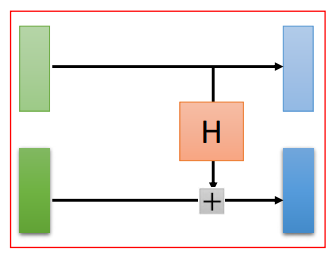
\includegraphics[height=0.4\textheight, width=\textwidth, keepaspectratio]{images/norm-flow/nfm_nice.png}
            \end{figure}
        \end{itemize}
        \item The Jacobian determinant of this transformation is 1, which simplifies density computation.
    \end{itemize}
    \framebreak
    \item Multiple additive coupling layers are composed together, with different partitions in each layer.
    \item \textbf{Limitation:} The transformation is volume-preserving and cannot model changes in volume, which limits expressiveness.
    \item \textbf{Enhancement:} A final rescaling layer is applied to introduce volume changes:
    \begin{align*}
        x = s \odot z
    \end{align*}
    where $s$ is a scaling factor.
\end{itemize}
\end{frame}

\begin{frame}[allowframebreaks]{NICE - Results}
\begin{figure}
    \centering
    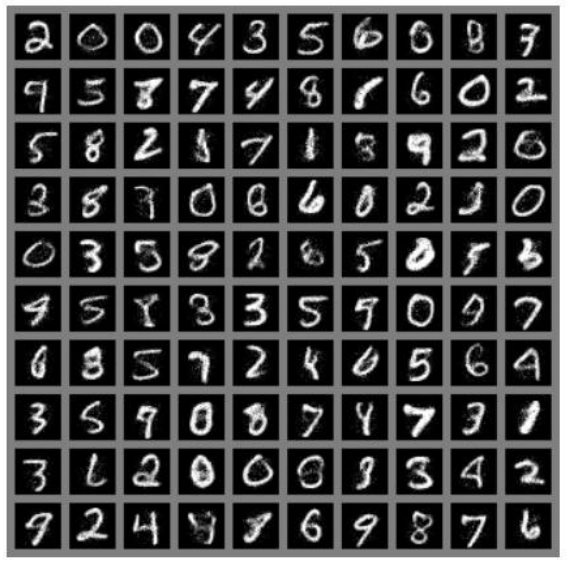
\includegraphics[height=0.8\textheight, width=\textwidth, keepaspectratio]{images/norm-flow/nfm_nice_mnist.png}
    \caption*{NICE generated samples when trained on the MNIST digits dataset.}
\end{figure}

\framebreak

\begin{figure}
    \centering
    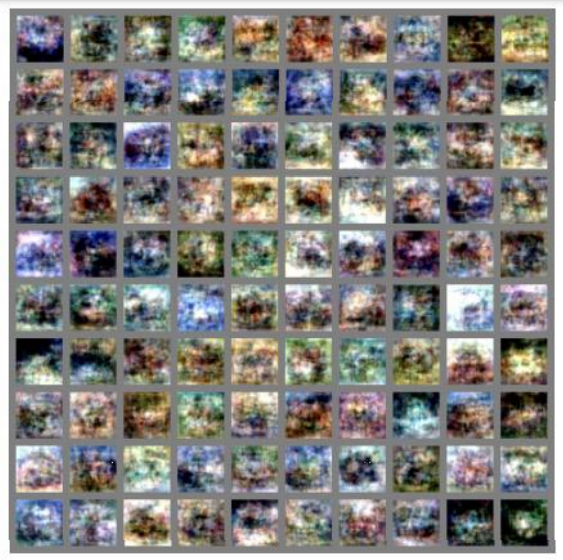
\includegraphics[height=0.8\textheight, width=\textwidth, keepaspectratio]{images/norm-flow/nfm_nice_cifar.png}
    \caption*{NICE generated samples when trained on the CIFAR-10 dataset.}
\end{figure}
    
\end{frame}